\label{sec: optimization}
In the spirit of \cite{Alouges2013} and \cite{Alouges2017}, we follow the notion of swimming efficiency suggested by Lighthill \cite{Lighthill1952} and we adopt the following notion of optimality: \emph{energy minimizing strokes are the ones that minimize the kinematic energy dissipated while trying to reach a given net displacement} $\delta p \in \R^3 \times \so(3) \simeq \R^6$. Mathematically speaking, the total energy dissipation due to a stroke $\xi \in H^1_{\sharp}(J, \R^4)$ can be evaluated through an adequate quadratic energy functional, c.f. \cite{Alouges2013},
\begin{equation}
 \mathcal{G}(\xi) := \int_{J} \mathfrak{g}(\xi(t))\dot{\xi}(t) \cdot \dot{\xi}(t) \dd t,
\end{equation}
where the energy density $\mathfrak{g} \in C^1(\R^{4 \times 4})$ is a function with values in the space of symmetric and positive definite matrices $M_{4 \times 4}(\R)$. In the small stroke regime, we can approximate the energy density by $\mathfrak{g}(\xi) = \mathfrak{g}(0) + o(1)$, where $\mathfrak{g}(0) \in M_{4 \times 4}(\R)$ is symmetric and positive definite. More precisely,
\begin{equation}
\label{eq: linearized energy functional}
	\mathcal{G}(\xi) := \int_{J} Q_{\mathfrak{g}}(\dot{\xi}(t))\dd t,
\end{equation}
with $Q_{\mathfrak{g}}(\eta) := \mathfrak{g}(0)\eta \cdot \eta$. For the same symmetry reasons as discussed in section \ref{sec: symmetries}, we necessarily have for all $\eta \in \R^4$
\begin{eqnarray}
	Q_{\mathfrak{g}}(P_{ij} \eta) = Q_{\mathfrak{g}}(\eta), & &\forall i,j \in \N_4,
\end{eqnarray}
where $P_{ij}$ denotes the permutation matrix swapping the $i$-th and $j$-th entries. By direct computation, one finds that the symmetric positive matrix $G$ representing the quadratic form $Q_{\mathfrak{g}}$ is of the form
\begin{equation}
G = \left ( \begin{array}{cccc}
\kappa & h & h & h \\ 
h & \kappa & h & h \\ 
h & h & \kappa & h \\ 
h & h & h & \kappa
\end{array} \right ),
\end{equation}
for two parameters $h$ and $\kappa > \max(h, -3h)$. In particular, we observe that $G \tau_k = (\kappa - h ) \tau_k$ for $k \in  \N_3$ and $G \tau_4 = (\kappa + 3h) \tau_4$. In the following, we denote by $\mathfrak{g}_1 := \mathfrak{g}_2 := \mathfrak{g}_3 := \kappa - h$ and $\mathfrak{g}_4 := \kappa + 3h$ the eigenvalues of $G$. Furthermore, the eigenvalues $(\mathfrak{g}_i)_{i \in \N_4}$ allow us to diagonalize  $G$ as
\begin{eqnarray}
G = U \Lambda_{\mathfrak{g}} U^T, & U := [\tau_1 | \tau_2 |\tau_3 |\tau_4], & \Lambda_{\mathfrak{g}} := \diag(\mathfrak{g}_i).
\end{eqnarray}

The goal of this section is to find a stroke $\xi \in \strokes$ minimizing $\mathcal{G}$ subject to a prescribed net displacement $\delta p \in \R^6$, i.e. subject to the constraint (c.f. (\ref{eq: net displacement}))
\begin{equation}
\label{eq: constraint}
\begin{aligned}
	 \delta p = \mathfrak{h}_{c} \sum_{k \in \N_3}\left ( \int_{J} \det( \xi(t) | \dot{\xi}(t) | \tau_{k+1} | \tau_{k+2}) \dd t \right ) f_k\\
	+ \mathfrak{h}_{\theta}  \sum_{k \in \N_3}\left ( \int_{J} \det ( \xi(t) | \dot{\xi}(t) | \tau_{k} | \tau_{4}) \dd t\right ) f_{k + 3}.
\end{aligned}
\end{equation}
Note that existence of such solutions follows readily by the direct method of variational calculus.


\subsection{Bivectors in four dimensions}
\label{sec:bivectors}
Let us recall in this section the basic definitions around the notion of \emph{bivectors}, where we refer to \cite{Lounesto2006} for details. Since the abstract definition of general $k$-vectors is not very useful for our purposes, we merely illustrate them in $\R^3$, which then generalizes easily to higher dimensions. In $\R^3$, a bivector is an oriented plane segment; that is, a small piece of surface having a magnitude given by the area of the surface element as well as a direction given by the attitude of the plane the surface element lies in as well as a sense of rotation. Together, they form the vector space $\bigwedge^2 \R^3$.
\begin{figure}[h]
    \centering
    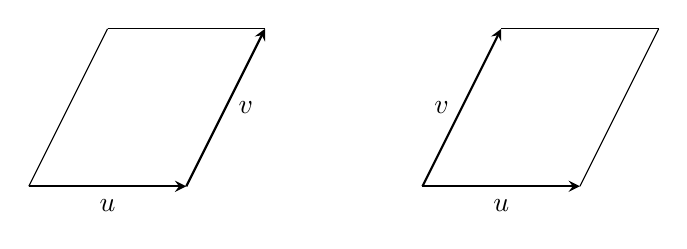
\begin{tikzpicture}[>=stealth]
    \draw[->, thick] (0,0) -- node[below=1pt] {$u$} (2,0);
    \draw (1,2) -- (3,2);
    \draw (0,0) -- (1,2);
    \draw[->, thick] (2,0) -- node[right=1pt] {$v$}(3,2);
    \draw[->, thick] (5,0) -- node[below=1pt] {$u$} (7,0);
    \draw (6,2) -- (8,2);
    \draw[->, thick] (5,0) -- node[left=1pt]{$v$} (6,2);
    \draw (7,0) -- (8,2);
    \end{tikzpicture}
    \caption{Sketch of a bivector $u \wedge v$ formed by sweeping $v$ along $u$ in contrast to the bivector $v \wedge u = - u \wedge v$, which is obtained by sweeping $u$ along $v$.}
    \label{fig:bivectors}
\end{figure}
We can represent a bivector $\omega \in \bigwedge^2 \R^3$ as a small parallelogram which suggests that we can think of it as some product of the two vectors along its sides, see figure \ref{fig:bivectors}. This is realized by the \emph{exterior product}, also called \emph{wedge product}, $u \wedge v$ of two vectors $u$ and $v$. The product $u \wedge v$ then represents the bivector obtained by sweeping $v$ along $u$. This operation yields a direct link between $\R^3$ and the vector space $\bigwedge^2 \R^3$ of bivectors, a basis of which is given by
\begin{equation}
 \{\hat{e}_1 \wedge \hat{e}_2, \hat{e}_1 \wedge \hat{e}_3, \hat{e}_2 \wedge \hat{e}_3\},
\end{equation}
if $\{\hat{e}_1, \hat{e}_2, \hat{e}_3\}$ is a basis of $\R^3$. In fact, the standard scalar product on $\R^3$ extends to a scalar product on $\bigwedge^2 \R^3$ by
\begin{equation}
( u_1 \wedge u_2 , v_1 \wedge v_2 ) = \det \left (\begin{array}{cc}
u_1 \cdot v_1 & u_1 \cdot v_2 \\ 
u_2 \cdot v_1 & u_2 \cdot v_2
\end{array}  \right).
\end{equation}
In particular, $( u \wedge v, u \wedge v ) = |u|^2 |v|^2 \sin^2\psi$, where $\psi$ is the angle between the vectors $u$ and $v$. Eventually, the norm of a bivector $\omega = \omega_{12} \hat{e}_1 \wedge \hat{e}_2 + \omega_{13} \hat{e}_1 \wedge \hat{e}_3 + \omega_{23} \hat{e}_2 \wedge \hat{e}_3$ is given by
\begin{equation}
|\omega| = \sqrt{\omega_{12}^2 + \omega_{13}^2 + \omega_{23}^2}.
\end{equation}
These definitions then extend naturally to all higher dimensions. In particular, we note that if $\{e_1, e_2, e_3, e_4\}$ again denotes the canonical basis of $\R^4$, a basis of the space $\bigwedge^2 \R^4$ is given by
\begin{equation}
\{e_{12}, e_{13}, e_{14}, e_{23}, e_{24}, e_{34}\},
\end{equation}
where we write $e_{ij} := e_i \wedge e_j$ to simplify notation.

To finish this section, we will point out some properties of the space $\bigwedge^2 \R^4$ and how it differs from $\bigwedge^2 \R^3$, which at a later point will illustrate why the optimal control curves for $\textsc{SPr3}$ and \textsc{SPr4} in general do not have the same structure.

As a matter of fact, one peculiarity of the bivectors in $\R^3$ is that they are isomorphic to the space $\R^3$ itself. This is realized by the so-called \emph{Hodge dual operator} $\star$, c.f. \cite{Lounesto2006} p. 38, which is defined in a way such that for any two vectors $u,v \in \R^3$ one has
\begin{equation}
\label{eq: hodge star}
u \wedge v = \star(u \times v),
\end{equation}
where $\times$ denotes the usual cross product. This entails two things: First, every bivector in $\R^3$ is \emph{simple}; that is, it can be written as the wegde product of two vectors. Second, every bivector in $\R^3$ defines one unique plane in $\R^3$. It is due to this underlying geometrical fact that the optimal control curves of \textsc{SPr3} are planar.

In contrast, in $\R^4$, the geometry of its bivectors proves to be more involved. As $\dim \bigwedge^2 \R^4 = 6$, it is clear that the bivectors in $\R^4$ are not isomorphic to $\R^4$ itself. In particular, in $\R^4$ not all bivectors are simple. Indeed, the bivector $e_1 \wedge e_2 + e_3 \wedge e_4 \in \bigwedge^2 \R^4$ cannot be written as an exterior product of just two vectors in $\R^4$. Nevertheless, any bivector in $\R^4$ can be written as the sum of two orthogonal simple bivectors \cite{Lounesto2006}. Moreover, we have the following criterion to determine whether a bivector is simple:


\begin{lemma}
\label{lem:simple bivector}
A bivector $\omega \in \bigwedge^2 \R^4$ is simple if and only if $\omega \wedge \omega = 0$.
\end{lemma}

\begin{proof}
If $\omega \in \bigwedge^2 \R^4$ is a simple bivector, i.e. if there are vectors $u,v \in \R^4$ such that $\omega = u \wedge v$, then it is clear from the anticommutativity and associativity of the wedge product that
\begin{equation}
\omega \wedge \omega = (u \wedge v) \wedge (u \wedge v) = - u \wedge u \wedge v \wedge v = 0.
\end{equation}
The inverse requires a rather lengthy proof by induction, see the lecture notes on projective geometry by Nigel Hitchin, chapter 3, p.48 \cite{Hitchin2003}.
\end{proof}

In what follows, we will find that the net displacement actually identifies with a bivector of $\R^4$. The solution to the optimization problem in \cite{Alouges2017} then suggests that we should be able to find a similar solution for our optimization problem, at least in the case where the net displacement is a simple bivector. The preceding lemma then serves us to identify certain subspaces of $\bigwedge^2 \R^4$ consisting only of simple bivectors. The structure of $\bigwedge^2 \R^4$ will nonetheless be crucial for the solution in the general case as well. The fact that every bivector represents in some sense two planes in $\R^4$ will indeed be the reason for the introduction of a second Fourier mode in the optimal strokes.

\subsection{G-Orthogonalization}
We begin by rewriting the energy functional (\ref{eq: linearized energy functional}) and the constraint (\ref{eq: constraint}) in terms of the orthonormal basis of eigenvectors $(\tau_i)_{i \in \N_4}$ of the matrix $G$. The change of variable $\eta(t) := U^T \xi(t) \in H_{\sharp}^{1}(J, \R^4)$, allows us to write
\begin{equation}
\label{eq: G-orth energy functional}
\mathcal{G}_{U}(\eta) = \int_{J} \Lambda_{\mathfrak{g}} \dot{\eta}(t) \cdot \dot{\eta}(t) \dd t,
\end{equation}
with $\mathcal{G}_{U}(\eta) := \mathcal{G}(\xi) = \mathcal{G}(U \eta)$. For the constraint, we note that
\begin{equation}
\det(\xi |\dot{\xi} | \tau_i | \tau_j) =  \det U \det (\eta | \dot{\eta} | e_i | e_j) = \det(\dot{\eta} | \eta | e_i |e_j),
\end{equation}
since $\det U = -1$. Eventually, we can express the determinants more elegantly in terms of exterior products. In fact, by direct calculation one obtains $\det(\dot{\eta} | \eta | e_k |e_4) = (\dot{\eta} \wedge \eta, e_{k + 1} \wedge e_{k+2})$ and $\det(\dot{\eta} |\eta | e_{k + 1} |e_{k + 2}) = (\dot{\eta} \wedge \eta, e_k \wedge e_4)$, for $k \in \N_3$ taken mod 3. Then, the isomorphism sending the standard basis $\{f_i\}_{i \in \N_6}$ of $\R^6$ onto the ordered basis 
\begin{equation}
\label{eq: basis of bivectors}
(e_{14}, e_{24}, e_{34}, e_{23}, e_{31}, e_{12})
\end{equation}
of $\bigwedge^2 \R^4$, where we write $e_{ij} := e_i \wedge e_j$, allows us to rewrite (\ref{eq: constraint}) as
\begin{equation}
\label{eq: G-orth constraint}
\Lambda_{\mathfrak{h}}^{-1} \delta p = \int_{J} \dot{\eta}(t) \wedge\eta(t) \dd t,
\end{equation}
with $\Lambda_{\mathfrak{h}} := \diag(\mathfrak{h}_{c}, \mathfrak{h}_{c}, \mathfrak{h}_{c}, \mathfrak{h}_{\theta}, \mathfrak{h}_{\theta}, \mathfrak{h}_{\theta})$.

\subsection{Fourier transformation of the minimization problem}
We denote by $\ell^2(\R^4)$ the space of sequences $\mathbf{u} := (u_n)_{n \in \N}$ in $\R^4$ such that the norm
\begin{equation}
	||\mathbf{u}||_{\ell^2(\R^4)} := \sqrt{ \sum_{n \in \N} |u_n|^2 }
\end{equation}
is finite. Consequently, we denote by $\dot{\ell}^2(\R^4)$ the Hilbert space of sequences $\mathbf{u} = (u_n)_{n \in \N} \in \ell^2(\R^4)$ such that $(n u_n)_{n \in \N} \in \ell^2(\R^4)$. As the elements in $H_{\sharp}^{1}(J, \R^4)$ are $2\pi$-periodic, we can express $\eta$ in terms of its Fourier series as
\begin{equation}
\eta(t) := \sum_{n \in \N} \cos(nt) a_n + \sin(n t) b_n,
\end{equation}
with $(a_n, b_n)_{n \in \N} \in \dot{\ell}^2(\R^4) \times \dot{\ell}^2(\R^4)$. Substitution of the Fourier series of $\dot{\eta}$ into the energy functional (\ref{eq: G-orth energy functional}) yields due to Parseval's equality
\begin{align}
\mathcal{G}_{U} (\eta) := \int_{J} \Lambda_{\mathfrak{g}} \dot{\eta}(t) \cdot \dot{\eta} dt &= \pi \sum_{n  \in \N} n^2(\Lambda_{\mathfrak{g}} a_n \cdot a_n + \Lambda_{\mathfrak{g}} b_n \cdot b_n) \\  &=
\frac{1}{2} ||\mathbf{u}||_{\ell^2(\R^4)}^2 + \frac{1}{2} ||\mathbf{v}||_{\ell^2(\R^4)}^2,
\end{align}
where we have set
\begin{align}
\label{eq:relation Fourier coeffs of eta}
	\mathbf{u} := (u_n)_{n \in \N} := \sqrt{2 \pi \Lambda_{\mathfrak{g}}}(n a_n)_{n \in \N} \text{ and } \mathbf{v} := (v_n)_{n \in \N} := \sqrt{2 \pi \Lambda_{\mathfrak{g}}} (n b_n)_{n \in \N}.
\end{align}
Clearly, we have $(\mathbf{u}, \mathbf{v}) \in \ell^2(\R^4) \times \ell^2(\R^4)$. As a result of the $L_{\sharp}^2(J, \R^4)$-orthogonality of the Fourier trigonometric system, we can express the constraint (\ref{eq: G-orth constraint}) in terms of Fourier coefficients as $2 \pi \sum_{n \in \N} \tfrac{1}{n} (nb_n) \wedge (n a_n) = \Lambda_{\mathfrak{h}}^{-1} \delta p$. Returning to our old notation for a moment, we note that for any $n \in \N$, we have
\begin{equation}
2 \pi n^2 \det(b_n | a_n | e_i | e_j) = \frac{\sqrt{\mathfrak{g}_i \mathfrak{g}_j}}{\sqrt{\det \Lambda_{\mathfrak{g}}}} \det(v_n | u_n |e_i | e_j),
\end{equation}
and hence by setting $\tilde{\Lambda}_{\mathfrak{g}} := \diag(\mathfrak{g}_c, \mathfrak{g}_c, \mathfrak{g}_c, \sqrt{\mathfrak{g}_c \mathfrak{g}_{\theta}}, \sqrt{\mathfrak{g}_c \mathfrak{g}_{\theta}}, \sqrt{\mathfrak{g}_c  \mathfrak{g}_{\theta}})$, with $\mathfrak{g}_1 :=\mathfrak{g}_2 := \mathfrak{g}_3 := \mathfrak{g}_c$ and $\mathfrak{g}_4 := \mathfrak{g}_\theta$, we eventually find
\begin{equation}
\label{eq:relation between net displacement and Fourier modes}
\sqrt{\det \Lambda_{\mathfrak{g}}} (\Lambda_{\mathfrak{h}} \tilde{\Lambda}_{\mathfrak{g}})^{-1} \delta p = \sum_{n \in \N} \frac{v_n  \wedge u_n}{n}.
\end{equation}
We thus have proved the following

\begin{proposition}
\label{prop: l2-minimization}
The $\strokes$ minimization of the functional $\mathcal{G}_U$ given by (\ref{eq: G-orth energy functional}) under the constraint (\ref{eq: G-orth constraint}) is equivalent to the minimization of the functional
\begin{equation}
\label{eq:l2-energy}
	\mathcal{F}(\mathbf{u}, \mathbf{v}) := \frac{1}{2} ||\mathbf{u} ||^2_{\ell^2(\R^4)} + \frac{1}{2} ||\mathbf{v}||^2_{\ell^2(\R^4)},
\end{equation}
defined in the product Hilbert space $\ell^2(\R^4) \times \ell^2(\R^4)$ and subject to the constraint
\begin{equation}
\label{eq:l2-constraint}
\sum_{n \in \N} \frac{1}{n} v_n \wedge u_n = \omega \text{ with } \omega := \sqrt{\det \Lambda_{\mathfrak{g}}}(\Lambda_{\mathfrak{h}} \tilde{\Lambda}_{\mathfrak{g}})^{-1} \delta p,
\end{equation}
where $\delta p \in \R^3 \times \so(3)$ is a prescribed net displacement of position and orientation.
\end{proposition}

We observe that we are in a very similar situation as in \cite{Alouges2017} with the fundamental difference however that this time the constraint is a bivector. Nevertheless, it is natural to try to generalize the approach in \cite{Alouges2017}, which in fact is true at least in the case of $\omega$ being simple. In particular, note that due to $\omega$ being related to $\delta p$ by a diagonal matrix, $\omega$ is simple if and only if $\delta p$ is simple.

\subsection[The simple case]{The simple case}
With the remarks from section \ref{sec:bivectors}, we are able to solve the constrained minimization problem of Proposition \ref{prop: l2-minimization} in a similar manner to \cite{Alouges2017} whenever the net displacement is a simple bivector. In fact, we retrieve essentially the same result, i.e. that the optimal control curves are ellipses in a certain plane defined by the net displacement. Let us prove

\begin{proposition}
\label{prop:simple reduction}
If $\omega$ is a simple bivector, then for any $(\mathbf{u}, \mathbf{v}) \in \ell^2(\R^4) \times \ell^2(\R^4)$ such that the constraint (\ref{eq:l2-constraint}) holds, there exist two vectors $u,v \in \R^4$ such that for the sequences $\mathbf{u}_{\star} := \mathbf{e}_1 u$ and $\mathbf{v}_\star := \mathbf{e}_1 v \in \ell^2(\R^4)$ one has 
\begin{equation}
\mathcal{F}(\mathbf{u_{\star}}, \mathbf{v_{\star}}) = \mathcal{F}(\mathbf{u}, \mathbf{v}) \text{ and } v \wedge u = \omega.
\end{equation}
\end{proposition}

\begin{proof}
If $\omega = 0$, then the proof is trivial. Thus, let us denote by $\hat{\omega}$ the unit bivector associated to $\omega$. For a couple $(\mathbf{u}, \mathbf{v}) \in \ell^2(\R^4) \times \ell^2(\R^4)$, we then choose $u,v \in \R^4$ such that the following relations hold:
\begin{eqnarray}
\label{eq:reduction int1}
	|u| = ||\mathbf{u} ||_{\ell^2(\R^4)}, &  |v| = ||\mathbf{v} ||_{\ell^2(\R^4)} , & \frac{v \wedge u}{|v \wedge u|} = \hat{\omega}.
\end{eqnarray}
The latter is possible since $\hat{\omega}$ is a simple bivector by hypothesis. Hence, there exist $x, y \in \R^4$ such that $\omega = x \wedge y$. Then we have for all $u, v \in \Span\{x,y\}$ such that $v \wedge u \neq 0$ that $v \wedge u/|v \wedge u| = \hat{\omega}$, up to permutation to account for the sign. Furthermore, we have $v \wedge u = ||\mathbf{u}||_{\ell^2(\R^4)} ||\mathbf{v}||_{\ell^2(\R^4)} (\sin\psi)\hat{\omega}$, where $\psi$ is the angle between $u$ and $v$. Therefore, the equality $v \wedge u = \omega$ can be satisfied by choosing the angle $\psi \in (0, \pi)$ such that
\begin{equation}
 \sin \psi = \frac{|\omega|}{||\mathbf{u}||_{\ell^2(\R^4)} ||\mathbf{v} ||_{\ell^2(\R^4)}}.
 \end{equation}
This is possible under the condition that the right hand side  of the previous equation is not greater than one. In fact, we have using the Cauchy-Schwarz inequality
\begin{equation}
|\omega| \leq \sum_{n \in \N} \frac{1}{n} |v_n \wedge u_n| \leq \sum_{n \in \N} |v_n| |u_n| \leq ||\mathbf{u} ||_{\ell^2(\R^4)} ||\mathbf{v} ||_{\ell^2(\R^4)}.
\end{equation}
Finally, from (\ref{eq:reduction int1}) we obtain
\begin{equation}
\mathcal{F}(\mathbf{u_\star}, \mathbf{v_{\star}}) = \frac{1}{2} |u|^2 + \frac{1}{2} |v|^2 = \frac{1}{2} ||\mathbf{u}||_{\ell^2(\R^4)}^2 + \frac{1}{2} ||\textbf{v}||_{\ell^2(\R^4)}^2,
\end{equation}
which concludes the proof.
\end{proof}

We immediately have

\begin{corollary}
\label{cor:simple reduction}
If $\omega$ is a simple bivector, the minimization problem for $\mathcal{F}$ in $\ell^2(\R^4) \times \ell^2(\R^4)$, under the constraint (\ref{eq:l2-constraint}), is equivalent to the minimization in $\R^4 \times \R^4$ of the function
\begin{equation}
\label{eq:finite dim energy}
 	f(u,v) := \frac{1}{2}|u|^2 + \frac{1}{2} |v|^2,
 \end{equation} 
 under the constraint
 \begin{equation}
 \label{eq:finite dim constraint}
 v \wedge u = \omega.
 \end{equation}
\end{corollary}

\begin{proof}
It suffices to observe that if $\mathcal{V}_{\omega}$ denotes the subset of $\ell^2(\R^4) \times \ell^2(\R^4)$ satisfying the constraint (\ref{eq:l2-constraint}) and by $V_{\omega}$ the subset of $(u, v)  \in \R^4 \times \R^4$ such that $v \wedge u = \omega$, then Proposition \ref{prop:simple reduction} yields
\begin{equation}
\min_{(\mathbf{u}, \mathbf{v}) \in \mathcal{V}_{\omega}}\mathcal{F}(\mathbf{u}, \mathbf{v}) = \min_{(u, v) \in V_\omega} \mathcal{F}(\mathbf{e}_1 u, \mathbf{e}_1 v) = \min_{(u,v) \in V_{\omega}} f(u,v).
\end{equation}
\end{proof}

Let us now prove the following


\begin{proposition}
\label{prop:finite dim minimization}
Any couple of vectors $(u_{\star}, v_{\star}) \in \R^4 \times \R^4$ minimizing the function $f$ given in (\ref{eq:finite dim energy}) and subject to the constraint (\ref{eq:finite dim constraint}) with $\omega = v \wedge u$ a simple bivector, is characterized by the following conditions:
\begin{eqnarray}
\label{eq:finite dim minimization conditions}
|u_{\star}|^2 = |v_{\star}|^2 = |\omega|, & 
u_{\star} \cdot v_{\star} = 0.
\end{eqnarray}
Therefore, any two vectors $\sigma, \mu \in \Span\{u, v\}$ such that $|\sigma|^2 = |\mu|^2 =|\omega|$ and $\sigma \cdot \mu = 0$, the couple $(\sigma, \mu) \in \R^4 \times \R^4$, up to permutation, is a (global) constrained minimizer for $f$.
\end{proposition}

\begin{remark}
To construct such a couple, it suffices to scale $v$ to get $v_\star$ and then find $u_\star$ by Gram-Schmidt orthogonalization and rescaling.
\end{remark}

\begin{proof}
Note that to find the minimizers of the problem (\ref{eq:finite dim energy}) - (\ref{eq:finite dim constraint}), the constraint $u \wedge v = \omega$ implies the existence of a $\psi \in (0, \pi)$ such that $|u||v| \sin \psi= |\omega|$. Hence, the constrained minimization for $f$ is equivalent to the unconstrained minimization of the function $\hat{f}: \R^4 \times (0, \pi) \to \R$ defined by
\begin{equation}
(u, \psi) \mapsto \frac{1}{2} |u|^2 + \frac{1}{2} \frac{|\omega|^2}{|u|^2 \sin^2\psi},
\end{equation}
whose stationary points satisfy $\psi_{\star} = \frac{\pi}{2}$ and $|u_{\star}|^2 = |\omega|$. This shows the necessity of the conditions stated in (\ref{eq:finite dim minimization conditions}). To show sufficiency of the condition, one observes that for any such points one has $\hat{f}(u_{\star}, \psi_{\star}) = |\omega|$. Indeed, for any $(u, \psi)  \in \R^4 \times (0, \pi)$ we have
\begin{equation}
\hat{f}(u, \psi) \geq \frac{1}{2} \frac{|u|^4 + |\omega|^2}{|u|^2} = |\omega| + \frac{1}{2}\frac{(|\omega| - |u|^2)^2}{|u|^2} \geq |\omega| = \hat{f}(u_{\star}, \psi_{\star}).
\end{equation}
A straightforward calculation shows then that for such $\sigma$ and $\mu$, one has $\sigma \wedge \mu \mid \mid \hat{\omega}$ since they are in the plane spanned by the vectors $u$ and $v$. By construction, one has $|\sigma \wedge \mu| = |\sigma| |\mu| = |\omega|$. In the case of $\sigma \wedge \mu = - \omega$, one just permutes the two vectors.
\end{proof}

Combining all the arguments above, we have our first optimality result:

\begin{theorem}
\label{thm:optimal control curves in the simple case}
Let $\delta p \in \R^3 \times \so(3) \simeq \bigwedge^2 \R^4$ be a prescribed net displacement. Moreover, assume that $\delta p$ identifies with a simple bivector. Then, any minimizer $\xi \in \strokes$ of the energy functional (\ref{eq: linearized energy functional}) subject to the constraint (\ref{eq: constraint}) is of the form
\begin{equation}
\xi(t) := (\cos t) a + (\sin t) b,
\end{equation}
i.e. an ellipse of $\R^4$ centered at the origin and contained in the plane spanned by the vectors $a$ and $b$. The vectors $a,b \in \R^4$ are obtained as follows:
\begin{enumerate}
\item We compute the vector $\omega$ via the relation
\begin{equation}
\omega := \diag \left (\frac{\sqrt{\mathfrak{g}_c \mathfrak{g}_{\theta}}}{\mathfrak{h}_c}, \frac{\sqrt{\mathfrak{g}_c \mathfrak{g}_{\theta}}}{\mathfrak{h}_c}, \frac{\sqrt{\mathfrak{g}_c \mathfrak{g}_{\theta}}}{\mathfrak{h}_c}, \frac{\mathfrak{g}_c}{\mathfrak{g}_\theta}, \frac{\mathfrak{g}_c}{\mathfrak{g}_\theta}, \frac{\mathfrak{g}_c}{\mathfrak{g}_\theta} \right ) \delta p \simeq v \wedge u,
\end{equation}
where we may assume that $u \cdot v = 0$ and $|u| = |v| = \sqrt{|\omega|}$.

\item We calculate the vectors $a$ and $b$ via the relations
\begin{equation}
\label{eq:global minimizer form}
\begin{aligned}
a := \frac{U \Lambda_{\mathfrak{g}}^{-1/2}}{\sqrt{2 \pi}} u,&& b := \frac{U \Lambda_{\mathfrak{g}}^{-1/2}}{\sqrt{2 \pi}} v.
\end{aligned}
\end{equation}
\end{enumerate}

In addition, the minimal value of the energy functional is $|\omega|$, and the vectors $a$ and $b$ are $\mathfrak{g}$-orthogonal, i.e. with respect to the inner product defined for every $x,y \in \R^4$ by $(x, y)_{\mathfrak{g}} := 2 \pi \Lambda_{\mathfrak{g}} x \cdot y$, and have the same $\mathfrak{g}$-norm $|a|_{\mathfrak{g}}^2 = |b|_{\mathfrak{g}}^2 = |\omega|$. 
\end{theorem}


\begin{proof}
From Proposition \ref{prop:finite dim minimization}, Corollary \ref{cor:simple reduction} and then Proposition \ref{prop: l2-minimization}, we get that any $u, v \in \R^4$ satisfying the relations
\begin{eqnarray}
v \wedge u = \omega,  &  u \cdot v = 0, &  |u|^2 = |v|^2 =  |\omega|,
\end{eqnarray}
 with $\omega := \sqrt{\det \Lambda_{\mathfrak{g}}} (\Lambda_{\mathfrak{h}} \tilde{\Lambda}_{\mathfrak{g}})^{-1} \delta p$, is associated to a (global) constrained minimizer for $\mathcal{G}_{U}$, via the curve $\eta(t) := (\cos t) \tilde{a} + (\sin t) \tilde{b}$, where the Fourier coefficients $\tilde{a}, \tilde{b} \in \R^4$ are related to $\omega$ (c.f. \ref{eq:relation Fourier coeffs of eta}) by $(\sqrt{2 \pi \Lambda_{\mathfrak{g}}}) \tilde{a} = u$ and $(\sqrt{2 \pi \Lambda_{\mathfrak{g}}}) \tilde{b} = v$. The minimum value of the energy is then $\mathcal{G}_{U}(\eta) = |\omega|$.

Finally, in the $\mathfrak{g}$-orthogonal reference frame, the inner product is defined by $(x, y)_{\mathfrak{g}} := 2 \pi \Lambda_{\mathfrak{g}}x \cdot y$ for $x,y \in \R^4$. Let us denote by $|\cdot|_{\mathfrak{g}}$ the associated norm. Then we have the following relations:
\begin{align}
|\tilde{a}|_{\mathfrak{g}}^2 = |\tilde{b}|_{\mathfrak{g}}^{2} = |\omega| \;  \text{ and } \; (\tilde{a}, \tilde{b})_{\mathfrak{g}} = 0.
\end{align}
Applying the orthogonal map $U$ to $\tilde{a}$ and $\tilde{b}$ finishes the proof.
\end{proof}

\subsubsection{Examples of simple net displacements}
In light of Theorem \ref{thm:optimal control curves in the simple case} presented above, one might ask whether there are concrete cases in which the net displacement happens to be a simple bivector. It turns out that there is convenient correspondence for engineering purposes between certain subspaces of $\bigwedge^2 \R^4$ consisting only of simple bivectors and certain net displacements. First, note that purely spatial net displacements are always simple since one can always factor out $e_4$ from all three corresponding basis vectors, cf. (\ref{eq: basis of bivectors}). Moreover, observe that the condition in Lemma \ref{lem:simple bivector} is in particular satisfied if all coefficients corresponding to a certain index are zero, e.g. $\omega_{i4} = 0$ for $i \in \N_3$. This yields four subspaces $D_{ijk} \subset \bigwedge^2 \R^4$ consisting only of simple bivectors. Then, by inspection of the basis of $\bigwedge^2 \R^4$, we find the correspondences displayed in table \ref{tab:simple net displacements}.
\begin{table}[h]
    \centering
        \begin{tabular}{cl}
        \toprule 
        \textit{Subspace} & \textit{Corresponding net displacements} \\ 
        \midrule 
        $D_{123}$ & rotations around all three axes  $\hat{e}_1, \hat{e}_2$, and $\hat{e}_3$ \\ 
        % \hline 
        $D_{124}$ & translation in the $\hat{e}_1\hat{e}_2$-plane, rotation around the $\hat{e}_3$-axis \\ 
        % \hline 
        $D_{134}$ & translation in the $\hat{e}_1\hat{e}_3$-plane, rotation around the $\hat{e}_2$-axis  \\ 
        % \hline 
        $D_{234}$ & translation in the $\hat{e}_2\hat{e}_3$-plane, rotation around the $\hat{e}_1$-axis  \\ 
        \bottomrule 
        \end{tabular} 
    \caption{Correspondences between subspaces of $\bigwedge^2 \R^4$ consisting of simple bivectors and net displacements in $\R^3\times \SO(3)$.}
    \label{tab:simple net displacements}
\end{table}

By comparison, the non-simple bivector $e_{12} + e_{34}$ corresponds to the net displacement $e_3 + L_3$, i.e. a screw motion. This kind of movement requires a solution to the general problem, which we treat in the following section.


\subsection{The general case}

Let us now address the case of a general net displacement, i.e. $\delta p \in \R^6 \simeq \bigwedge^2 \R^4$ which identifies to a non-simple bivector. Recall that every simple bivector represents a plane in $\R^4$, while we can always express an arbitrary bivector in $\bigwedge^2 \R^4$ as the sum of two orthogonal simple bivectors. Therefore, the observations from section \ref{sec:bivectors} suggest that the optimal curve in the general case consists of two ellipses in two planes. We will indeed be able to prove this result. However, we first have to return to variational calculus to do so.


\subsubsection{The optimization problem in the variational setting}
More precisely, we will establish the structure of the optimal control curves using the Euler-Lagrange equation associated with the optimization problem. To that end, let us recast the optimization problem in its original form:
\begin{align}
\label{eq:original_optimization_problem}
\begin{cases}
 \text{Find } \min_{\xi \in \dot{H}^1_{\sharp}} \int_{J} G \dot{\xi}(t) \cdot \dot{\xi}(t) \dd t\\
 \text{under the constraints }\\
 \int_{J} M_i \dot{\xi}(t) \cdot \xi(t) \dd t = \delta p_i,\, i \in \N_6.
 \end{cases}
\end{align}
Accordingly, we are in the setting of a variational problem with six isoperimetric constraints. For $i \in \N_6$, denote by $K_i: \strokes \times L^2_\sharp(J, \R^4) \times J \to \R$ the map
\begin{align}
	K_i(\xi, \eta, t) := M_i \eta(t) \cdot \xi(t).
\end{align}
Furthermore, denote by $\mathcal{K}_i : \strokes \to \R$ the functional
\begin{align}
	\mathcal{K}_i(\xi) := \int_{J} K_i(\xi, \dot{\xi}, t) \dd t.
\end{align}
Then, the six isoperimetric constraints read $\mathcal{K}_i(\xi) = \delta p_i$ for $i \in \N_6$. Now, let us denote by $\delta \mathcal{G}$ and $\delta \mathcal{K}_i$ the first variations of $\mathcal{G}$ and the $\mathcal{K}_i$, respectively. Then a slight adaptation of Proposition 2.1.3. in \cite{Kielhoefer2018} shows that $\xi \in \strokes$ is a minimizer of (\ref{eq:original_optimization_problem}) and if $\xi$ is not critical for the constraints, i.e. $\delta \mathcal{K}_1(\xi), \dotsc, \delta \mathcal{K}_6(\xi)$ are linearly independent, then $\xi$ satisfies the Euler-Lagrange equation:

\begin{align}
\label{eq:euler_lagrange}
\frac{\dd}{\dd t} \frac{\partial}{\partial \dot{\xi}} \left ( G \dot{\xi}(t) \cdot \dot{\xi}(t) + \sum_{i \in \N_6} \mu_i K_i(\xi, \dot{\xi}, t)\right ) = \frac{\partial}{\partial \xi} \left ( G \dot{\xi}(t) \cdot \dot{\xi}(t) + \sum_{i \in \N_6} \mu_i K_i(\xi, \dot{\xi}, t)\right ),
\end{align}
for some $\mu \in \R^6$. To make use use of equation (\ref{eq:euler_lagrange}), let us prove the following result.

\begin{proposition}
\label{prop:linearly_independent_constraints}
Let $\delta p \in \R^6 \simeq \bigwedge^2 \R^4$ be non-simple and $\xi \in \strokes$ a minimizer of (\ref{eq:original_optimization_problem}). Then the functionals $\delta \mathcal{K}_1(\xi), \dotsc, \delta \mathcal{K}_6(\xi)$ are linearly independent.
\end{proposition}

\begin{proof}
Let $\lambda_1, \dotsc, \lambda_6 \in \R$ be such that $\sum_{i \in \N_6} \lambda_i \delta \mathcal{K}_i(\xi) $ is the zero functional in the dual space of $\strokes$. Note that by the periodicity of $\xi$ and integration by parts, we have for any $h \in \strokes$ that
\begin{align}
	\delta \mathcal{K}_i(\xi) h =  2 \int_J M_i \dot{\xi}(t) \cdot h(t) \dd t.
\end{align}
Setting $\Omega(\lambda) := \sum_{i \in \N_6} \lambda_i M_i$ for $\lambda \in \R^6$, we find that the functional $h \in \strokes \mapsto \int_J \Omega(\lambda) \dot{\xi}(t) \cdot h(t) \dd t$ is the zero functional. For the time being, let us choose $h = \Omega(\lambda) \dot{\xi}$, but note that $h$ is not necessarily in $\strokes$. Then we have
\begin{align}
\label{eq:zero_functional}
	0 = \int_J \Omega(\lambda) \dot{\xi}(t) \cdot h(t) \dd t = ||h||_{L^2}^{2},
\end{align}
i.e. $h \equiv 0$ almost everywhere. This can only happen in the two cases $\xi(t) \in \ker \Omega(\lambda)$ for all $t \in J$ or $\lambda_1 = \dotsm = \lambda_6 = 0$, in the latter of which we are done. So, let us suppose that we are in the former case. Note that the matrix $\Omega(\lambda)$ is skew symmetric. Hence, we find an orthogonal transformation $S$ such that $\Omega(\lambda) = S \Sigma(\lambda) S^T$ with

\begin{align}
\Sigma(\lambda) = \diag \left (\left( \begin{array}{cc}
0 & \nu_+(\lambda) \\ 
- \nu_+ (\lambda) & 0
\end{array} \right ) , \left ( \begin{array}{cc}
0 & \nu_{-}(\lambda) \\ 
- \nu_{-}(\lambda) & 0
\end{array} \right ) \right ).
\end{align}
Denoting by $P$ and $Q$ the projections $\R^6 \to \R^3$ on the first respectively the last three coordinates, the scalars $\nu_{\pm}$ are given by
\begin{align}
	\nu_{\pm} = 2 \sqrt{3} \sqrt{A \pm \sqrt{A^2 - K}},
\end{align}
with $A := \alpha^2 |P \lambda|^2 + \delta^2 |Q \lambda|^2$ and $K := 4 \alpha^2 \delta^2 |P\lambda \cdot Q \lambda|^2$. Hence, only $\nu_-$ can vanish, which implies that $\ker \Omega(\lambda)$ is at most of dimension two. However, this is excluded by the Lemma below, as $\delta p$ is assumed to be non-simple. Thus, we have $||h||_{L^2} > 0$. Now, approximation of $\dot{\xi}$ by smooth functions shows that $h \in \strokes \mapsto \int_J \Omega(\lambda) \dot{\xi}(t) \cdot h(t) \dd t$ cannot be the zero functional. Therefore, we must have $\lambda_1 = \dotsm = \lambda_6 = 0$, which finishes the proof.
\end{proof}

The following Lemma completes the proof of Proposition \ref{prop:linearly_independent_constraints}:
\begin{lemma}
	Let $\xi \in \strokes$ be a control curve. Suppose that $\xi(t) \in D$ for all $t \in J$, where $D \subset \R^4$ is a plane through the origin. Then, the net displacement due to $\xi$ is a simple bivector.
\end{lemma}

\begin{proof}
Note that if $\xi$ only takes values in the plane $D$, then the rescaled Fourier coefficients in relation (\ref{eq:l2-constraint}) must also lie in a plane $D'$ (not necessarily the same). Hence, the net displacement due to $\xi$ lies in fact in $\bigwedge^2 D'$. Thus, it must be simple since $D'$ is of dimension two and consequently $\dim \bigwedge^2 D' = 1$.
\end{proof}

\subsubsection{Structure of the solutions to the Euler-Lagrange equation}

By direct computation, one finds that after integration and utilizing the fact that $\xi$ is of average zero, the Euler-Lagrange equation (\ref{eq:euler_lagrange}) reads
\begin{equation}
\label{eq:euler_lagrange_integrated}
G \dot{\xi} - \Omega(\mu) \xi = 0,
\end{equation}
where $\Omega(\mu)$ is the skew symmetric matrix from (\ref{eq:zero_functional}). To reveal the structure of the solutions to (\ref{eq:euler_lagrange_integrated}), we need to apply two basis transformations: First, setting $\eta := G^{1/2} \xi$ yields
\begin{equation}
\dot{\eta} - \tilde{\Omega}(\mu) \eta = 0,
\end{equation}
where $\tilde{\Omega}(\mu) := \sum_{i \in \N_6} \mu_i G^{-1/2} M_i G^{-1/2}$, which is still a skew symmetric matrix. Hence, we find an orthogonal transformation $Q$ such that $\tilde{\Omega} = Q \tilde{\Sigma}(\mu) Q^T$ with
\begin{align}
	\tilde{\Sigma}(\mu) \diag \left (\left( \begin{array}{cc}
0 & \sigma_1(\mu) \\ 
- \sigma_1(\mu) & 0
\end{array} \right ) , \left ( \begin{array}{cc}
0 & \sigma_2(\mu) \\
- \sigma_2(\mu) & 0
\end{array} \right ) \right ).
\end{align}
Consequently, setting $\phi := Q \eta$, we have the equation $\dot{\phi} = \tilde{\Sigma}(\mu) \phi$, the solution of which is given by $\phi(t) = \exp \left ( \tilde{\Sigma}(\mu) t \right )\phi_0$ with $\phi_0 := QG^{1/2}\xi(0)$. By defining the vectors
\begin{align}
	\phi_{\sigma_1} &:= (\phi_{0,1}, \phi_{0,2}, 0, 0)^T,  & \psi_{\sigma_1} &:= (\phi_{0,2}, - \phi_{0,1}, 0, 0)^T,\\
	\phi_{\sigma_2} &:= (0,0,\phi_{0,3}, \phi_{0, 4})^T,  & \psi_{\sigma_2} &:= (0,0,- \phi_{0,4}, \phi_{0,3})^T,
\end{align}
and explicitly calculating $\exp(\tilde{\Sigma}(\mu)t)$, we can recast the curve $\phi$ as
\begin{eqnarray}
\phi(t) = \sum_{i \in \N_2} [\cos(\sigma_i(\mu)t) \phi_{\sigma_i} + \sin(\sigma_i(\mu)t) \psi_{\sigma_i}], & & t \in J.
\end{eqnarray}
Resubstituting the basis transformations, we find that $\xi$ must be of the form
\begin{eqnarray}
\label{eq:general_optimal_curve}
\xi(t) = \sum_{i \in \N_2} [\cos(\sigma_i(\mu)t) a_{\sigma_i} + \sin(\sigma_i(\mu)t) b_{\sigma_i}], & & t \in J.
\end{eqnarray}
Note that the vectors $\phi_{\sigma_1}, \psi_{\sigma_1}, \phi_{\sigma_2}$ and $\psi_{\sigma_2}$ are pairwise orthogonal. So, $\phi$ is in fact a rotation in two completely orthogonal planes of $\R^4$. In particular, this implies that the vectors $a_{\sigma_1}, b_{\sigma_1}, a_{\sigma_2}$ and $b_{\sigma_2}$ are orthogonal in the reference system of $G$.

\subsubsection{Existence of integer eigenvalues}
It is clear that the eigenvalues $\sigma_1(\mu)$ and $\sigma_2(\mu)$ must be integers for the curve $\xi$ in (\ref{eq:general_optimal_curve}) to be periodic. Hence, we must be able to choose $\mu \in \R^6$ such that $\sigma_1(\mu), \sigma_2(\mu) \in \N$. This question is addressed in this subsection.

First, note that we cannot have $\sigma_1(\mu) = \sigma_2(\mu)$ since then there would be only one Fourier mode and thus the relation (\ref{eq:relation between net displacement and Fourier modes}) would imply that $\delta p$ is simple. Next, one finds that the eigenvalues are given by
\begin{align}
	\sigma_{1,2}(\mu) = \frac{2 \sqrt{3}}{g_c \sqrt{g_\theta}} \sqrt{A \mp \sqrt{A^2 - K}},
\end{align}
where this time $A := \alpha^2 g_c |P \mu|^2 + \delta^2 g_{\delta} |Q \mu|^2 \geq 0$ and $K := 4 \alpha^2 \delta^2 g_c g_\theta |P\mu \cdot Q \mu|^2 \geq 0$. Clearly, we have $\sigma_2(\mu) \geq \sigma_1(\mu)$. So let us find the values for $\mu \in \R^6$ such that
\begin{eqnarray}
\label{eq:integer_condition}
	\sigma_1(\mu) = k \in \N \text{ and } \sigma_2(\mu) = lk, & & l \in \N.
\end{eqnarray}
This does not cover all possible pairs of integers. However, we will see in the next subsection that this is sufficient.

Imposing the two equations above on the eigenvalues leads to the definition of the quadratic form associated to the positive definite matrix
\begin{align}
	\Gamma := \frac{48}{g_c^2 g_\theta} \left (\begin{array}{cc}
	\alpha^2 g_c I_3 & 0 \\ 
	0 & \delta^2 g_\theta I_3
	\end{array}  \right ).
\end{align}
Indeed, one can show that the solution sets to (\ref{eq:integer_condition}) are given by $E_+^{k,l} \cup E_{-}^{k,l}$, where
\begin{align}
E_+^{k,l} := \{\mu \in \R^6 \mid \Gamma \mu \cdot \mu = \tfrac{(1 + l^2)k^2}{l^2}\} \text{ and } E_{-}^{k,l} := \{\mu \in \R^6 \mid \Gamma \mu \cdot \mu = (1 + l^2)k^2\},
\end{align}
i.e. the solutions are the union of two specific ellipsoids in $\R^6$. Note in particular, that this calculation covers the case $\sigma_1(\mu) = 1$ and $\sigma_2(\mu) = 2$. So, we have assured the existence of periodic solutions to the Euler-Lagrange equation and we will show in the following subsection that the latter choice of values for the eigenvalues is indeed optimal.

\subsubsection{Optimal control curves}
As of yet, the geometric structure of the optimal control curves is clear from (\ref{eq:general_optimal_curve}). So, let us now settle their explicit construction from a given non-simple net displacement. To that end, let us transform the Fourier modes $a_{\sigma_1}, b_{\sigma_1}, a_{\sigma_2}$ and $b_{\sigma_2}$ to the $G$-orthogonal reference by setting $\tilde{a}_{\sigma_1} := U^Ta_{\sigma_1}$ and similarly for the others. Then, substituting the curve into the energy functional $G$ yields
\begin{align}
\label{eq:optimal_energy}
	\mathcal{G}(\xi) = \pi \sigma_1(\mu)^2[\Lambda_{\mathfrak{g}}\tilde{a}_{\sigma_1} \cdot \tilde{a}_{\sigma_1} + \Lambda_\mathfrak{g} \tilde{b}_{\sigma_1} \cdot \tilde{b}_{\sigma_1}] + \pi \sigma_2(\mu)^2[\Lambda_{\mathfrak{g}} \tilde{a}_{\sigma_2} \cdot \tilde{a}_{\sigma_2} + \Lambda_{\mathfrak{g}}\tilde{b}_{\sigma_2} \cdot \tilde{b}_{\sigma_2}]\\
	=\frac{\sigma_1(\mu)}{2} [|u_{\sigma_1}|^2 + |v_{\sigma_1}|^2] + \frac{\sigma_2(\mu)}{2}[|u_{\sigma_2}|^2 + |v_{\sigma_2}|^2],
\end{align}
with 
\begin{eqnarray}
\label{eq:relation of decomposition to Fourier coeffs}
	u_{\sigma_i} := \sqrt{2 \pi \sigma_i(\mu) \Lambda_\mathfrak{g}}\tilde{a}_{\sigma_i} &\text{ and }& v_{\sigma_i} := \sqrt{2 \pi \sigma_i(\mu) \Lambda_{\mathfrak{g}}} \tilde{b}_{\sigma_i},
\end{eqnarray}
for $i \in \N_2$. In particular, it follows from relation (\ref{eq:relation between net displacement and Fourier modes}) that
\begin{equation}
	\sqrt{\det \Lambda_{\mathfrak{g}}}(\Lambda_{\mathfrak{h}} \Lambda_{\mathfrak{g}})^{-1} \delta p = v_{\sigma_1} \wedge u_{\sigma_1} + v_{\sigma_2} \wedge u_{\sigma_2}.
\end{equation}
We observe that the latter relation in the sense of (\ref{eq:relation between net displacement and Fourier modes}) is independent of the indices $\sigma_1$ and $\sigma_2$.  So, we can choose $\sigma_1(\mu) = 1$ and $ \sigma_2(\mu) = 2$ up to permutation such that $|u_{\sigma_1}|^2 + |v_{\sigma_1}|^2 \geq |u_{\sigma_2}|^2 + |v_{\sigma_2}|^2$. This choice of frequencies minimizes the energy in (\ref{eq:optimal_energy}). Recall that it has been shown in the previous section, that we can indeed find $\mu \in \R^6$, which realizes $\sigma_1(\mu) = 1$ and $\sigma_2(\mu) = 2$

Moreover, note that the vectors $u_{\sigma_1}, v_{\sigma_1}, u_{\sigma_2},$ and $v_{\sigma_2}$ are pairwise orthogonal due to the $G$-orthogonality of $a_{\sigma_1}, b_{\sigma_1}, a_{\sigma_2},$ and $b_{\sigma_2}$. Eventually, due to the bilinearity of the exterior product, we can always suppose that $|u_{\sigma_1}| = |v_{\sigma_1}|$ and $|u_{\sigma_2}| = |v_{\sigma_2}|$, which then fully minimizes the energy. One can see this by slightly adapting Proposition \ref{prop:finite dim minimization}. Conversely, note that once we are given a decomposition of $\omega  = 	\sqrt{\det \Lambda_{\mathfrak{g}}}(\Lambda_{\mathfrak{h}} \Lambda_{\mathfrak{g}})^{-1} \delta p$ into the sum of two orthogonal simple bivectors, the equations in (\ref{eq:relation between net displacement and Fourier modes}) give us a direct relation between the prescribed net displacement and the Fourier coefficients of the optimal control curve. Finally, let us summarize the above argument as follows.

\begin{theorem}
\label{thm:optimal_control_curves_general_case}
Let $\delta p \in \R^6 \simeq \bigwedge^2 \R^4$ a net displacement identifying to a non-simple bivector, then the energy minimizing curve which attains $\delta p$ is given by
\begin{eqnarray}
\xi(t) := \cos(t) a_1 + \sin(t) b_1 + \cos(2t) a_2 + \sin(2t) b_2,& t \in J,
\end{eqnarray}
where the vectors $a_1, b_1,a_2, b_2 \in \R^4$ are determined as follows:
\begin{enumerate}
\item First, we decompose the bivector $\omega := \sqrt{\det \Lambda_{\mathfrak{g}}}(\Lambda_{\mathfrak{h}} \tilde{\Lambda}_{\mathfrak{g}})^{-1} \delta p$ into the sum of two orthogonal simple bivectors, i.e.
\begin{align}
	\omega = v_1 \wedge u_1 + v_2 \wedge u_2,
\end{align}
with  all four vectors $u_1, u_2, v_1, v_2$ pairwise orthogonal and  $|u_i| = |v_i|$, for $i \in \N_2$.

\item If necessary, we permute the indices such that $|u_2|^2 + |v_2|^2 \leq |u_1|^2 + |v_1|^2$.

\item We set
	\begin{align}
		a_1 := \frac{U \Lambda_{\mathfrak{g}}^{-1/2}}{\sqrt{2 \pi}} u_1 &, & b_1 := \frac{U \Lambda_{\mathfrak{g}}^{-1/2}}{\sqrt{2 \pi}}v_1,\\
	a_2 := \frac{U \Lambda_{\mathfrak{g}}^{-1/2}}{\sqrt{4 \pi}} u_2& , & b_2 := \frac{U \Lambda_{\mathfrak{g}}^{-1/2}}{\sqrt{4 \pi}} v_2.	
	\end{align}
\end{enumerate}
Then the four vectors $a_1, b_1, a_2, b_2$ are $\mathfrak{g}$-orthogonal and the minimum value of the energy functional is $\frac{1}{2} [|u_1|^2 + |v_1|^2] +  [|u_2|^2 + |v_2|^2]$.
\end{theorem}

\begin{remark}
We point out here that in the simple case, we automatically retrieve the result from Theorem \ref{thm:optimal control curves in the simple case}.
Note also that in the simple case, the energy consumed by a energy minimizing stroke $\xi_*$ was $\mathcal{G}(\xi_*) = |\omega|$ for $\omega = \sqrt{\det \Lambda_{\mathfrak{g}}}(\Lambda_{\mathfrak{h}} \tilde{\Lambda}_{\mathfrak{g}})^{-1} \delta p$. In the general case, where $\omega = v_1 \wedge u_1 + v_2 \wedge u_2$, where the four vectors are mutually orthogonal and $|u_i| = |v_i| := l_i$ for $i \in \N_2$, we have by the Pythagorean Theorem that $|w|^2 = |l_1|^4 + |l_2|^4$. So, for a minimizer $\xi_*$ of the general problem, we find the estimate $\mathcal{G}(\xi_*) = l_1^2 + 2 l_2^2 \leq 3 |\omega|$. This allows us to frame the energy consumption by minimizing control curves in terms of the norm of the net displacement.
\end{remark}

\subsubsection{Non-uniqueness of optimal curves}
\label{subsec:non_uniqueness}
To end this section, we want to highlight a striking feature of the control system associated to the swimmer \textsc{SPr4}, namely that the optimal control curves are not necessarily unique. This follows readily from the fact that the decomposition of a bivector $\omega \in \bigwedge^2 \R^4$ into the sum of two orthogonal simple bivectors is not unique when the norms of the two summands are equal \cite{Lounesto2006}. Indeed, consider the net displacement $\delta p \in \R^3 \times \so(3) \simeq \bigwedge^2 \R^4$ such that
\begin{equation}
    \omega =  \sqrt{\det \Lambda_{\mathfrak{g}}}(\Lambda_{\mathfrak{h}} \tilde{\Lambda}_{\mathfrak{g}})^{-1} \delta p = e_1 \wedge e_2 + e_3 \wedge e_4.
\end{equation}
Clearly, the two summands on the right hand side are of equal norm. In fact, we have the second equation
\begin{equation}
\label{eq:non_unique_decomposition}
    \omega = e_1 \wedge e_2 + e_3 \wedge e_4 = \tfrac{1}{2}(e_1 + e_3) \wedge (e_2 + e_4) + \tfrac{1}{2}(e_1 - e_3)\wedge(e_2 - e_4).
\end{equation}
Hence, the construction in Theorem \ref{thm:optimal_control_curves_general_case} yields two distinct control curves which realize the same net displacement using the same (optimal) amount of energy. The different trajectories of \textsc{SPr4} due to the two distinct optimal control curves in the limit of very long arms are displayed in figure \ref{fig:non_unique_curves}, where we had to rescale $\delta p$ appropriately, for details see sections \ref{sec:laa} and \ref{sec:numerics}.
\begin{figure}[h]
    \centering
    \includegraphics[width = \textwidth]{images/non_unique_curves.png}
    \caption{The tractectories of \textsc{SPr4} in the limit of very long arms due to the two distinct optimal control curves resulting from the two decompositions in (\ref{eq:non_unique_decomposition}), shown (from left to right) in frontal view, side view and top view. The red trajectory corresponds to the left decomposition, while the blue trajectory corresponds to the right one.}
    \label{fig:non_unique_curves}
\end{figure}



